\input{problemSetSettings.tex}
\input{thesisDefs.tex}
\input{qftDefs.tex}

\def\hbac{\ensuremath{\text{HbA}_\text{1c}}}
\def\mgdl{\ensuremath{\text{mg/dL}}}
\def\sens{$\mgdl\over{U}$}
\def\carbratio{\ensuremath{R_\text{I-C}}}
\def\ric{\carbratio}
\def\rbas{\ensuremath{R_\text{Bas}}}

%\title{QFT I Homework 3}
%\author{Kurt Brendlinger}
%\date{}

\begin{document}
%\maketitle
\thispagestyle{empty}
\noindent {\bf Kurt Brendlinger - BGSuggest TDR}
%%%%%%%%%%%%%%%%%%%%%%%%%%%%%%%%%%%%%%%%%%%%
%%%%%%%%%%%%%%%%%%%%%%%%%%%%%%%%%%%%%%%%%%%%
%%%%%%%%%%%%%%%%%%%%%%%%%%%%%%%%%%%%%%%%%%%%
\section{Scope of this document}

The purpose of this document is to lay a basic foundation for a semi-automated fast-acting insulin 
dosage suggestion system, based on personal data collected by the Minimed Paradigm insulin pump and 
its associated blood glucose meter. By collecting and analyzing insulin dosages (including basal 
rates, food boluses and correction boluses), food intake, and other behavioral information from a 
specific user, the software (hereafter referred to as BGSuggest) will seek to suggest changes to 
the user's insulin regime in as focused a manner as possible.

While an idealized version of the software would require no additional feedback from the user other 
than a dedicated log of food and insulin intake, it is expected that early versions of this software 
will require the user to perform certain specific tasks (such as fasting basal tests).

Furthermore, it is anticipated that the software development will proceed in stages. In order to 
quickly produce results, a first tool will use aggregate information to make suggestions, in a 
brute-force approach which ignores some nuances (Phase I). While this tool may be effective at 
lowering average blood sugar rates, it is susceptible to the effects of localized events, including 
meal carbohydrate uncertainties, exercise, and fatty meals.

A second tool, aimed at evaluating data event-by-event, allows for more precise feedback. By 
analyzing data event-by-event, and incorporating meal carbohydrate estimate uncertainties, it would 
be able to suggest changes on an event-by-event basis, with appropriate uncertainties. The problem 
with this approach is that incorrect dosages can be blamed on any of three (or more) sources, and 
thus in a single event the data is under-constrained. The problem is resolved with three or more 
measurements; however, three accurate measurements within the same hour of the day is sometimes 
difficult, and the degree of uncertainty may be high. It is envisioned that the Phase II tool would 
leave these ambiguities unresolved, and up to the discretion of the user.

A third tool (Phase III) would attempt to solve this problem by attempting to minimize some 
converging test statistic through varying the three dosage variables (basal, bolus, sensitivity). To 
develop this tool, some truth studies may be helpful.

Other related tools could be imagined, such as a tool to recognize trends in certain meal types (or 
even a particular food) and suggest changes to carbohydrate estimation. These tools would require a 
dedicated user whose blood sugar levels were already known to a fairly precise level, and whose carb 
counting techniques were well-honed.

Before Phase I can begin, however, a basis of plotting and visualization techniques, as well as a 
system of persistified data (ntuples) must be devised (Phase 0).

This document will also serve as a repository of information, researched and anecdotal, related to 
balancing an maintaining blood sugar rates.

%%%%%%%%%%%%%%%%%%%%%%%%%%%%%%%%%%%%%%%%%%%%
%%%%%%%%%%%%%%%%%%%%%%%%%%%%%%%%%%%%%%%%%%%%
%%%%%%%%%%%%%%%%%%%%%%%%%%%%%%%%%%%%%%%%%%%%

\section{Phase 0 Software}

\begin{figure}[htbp]
\begin{center}
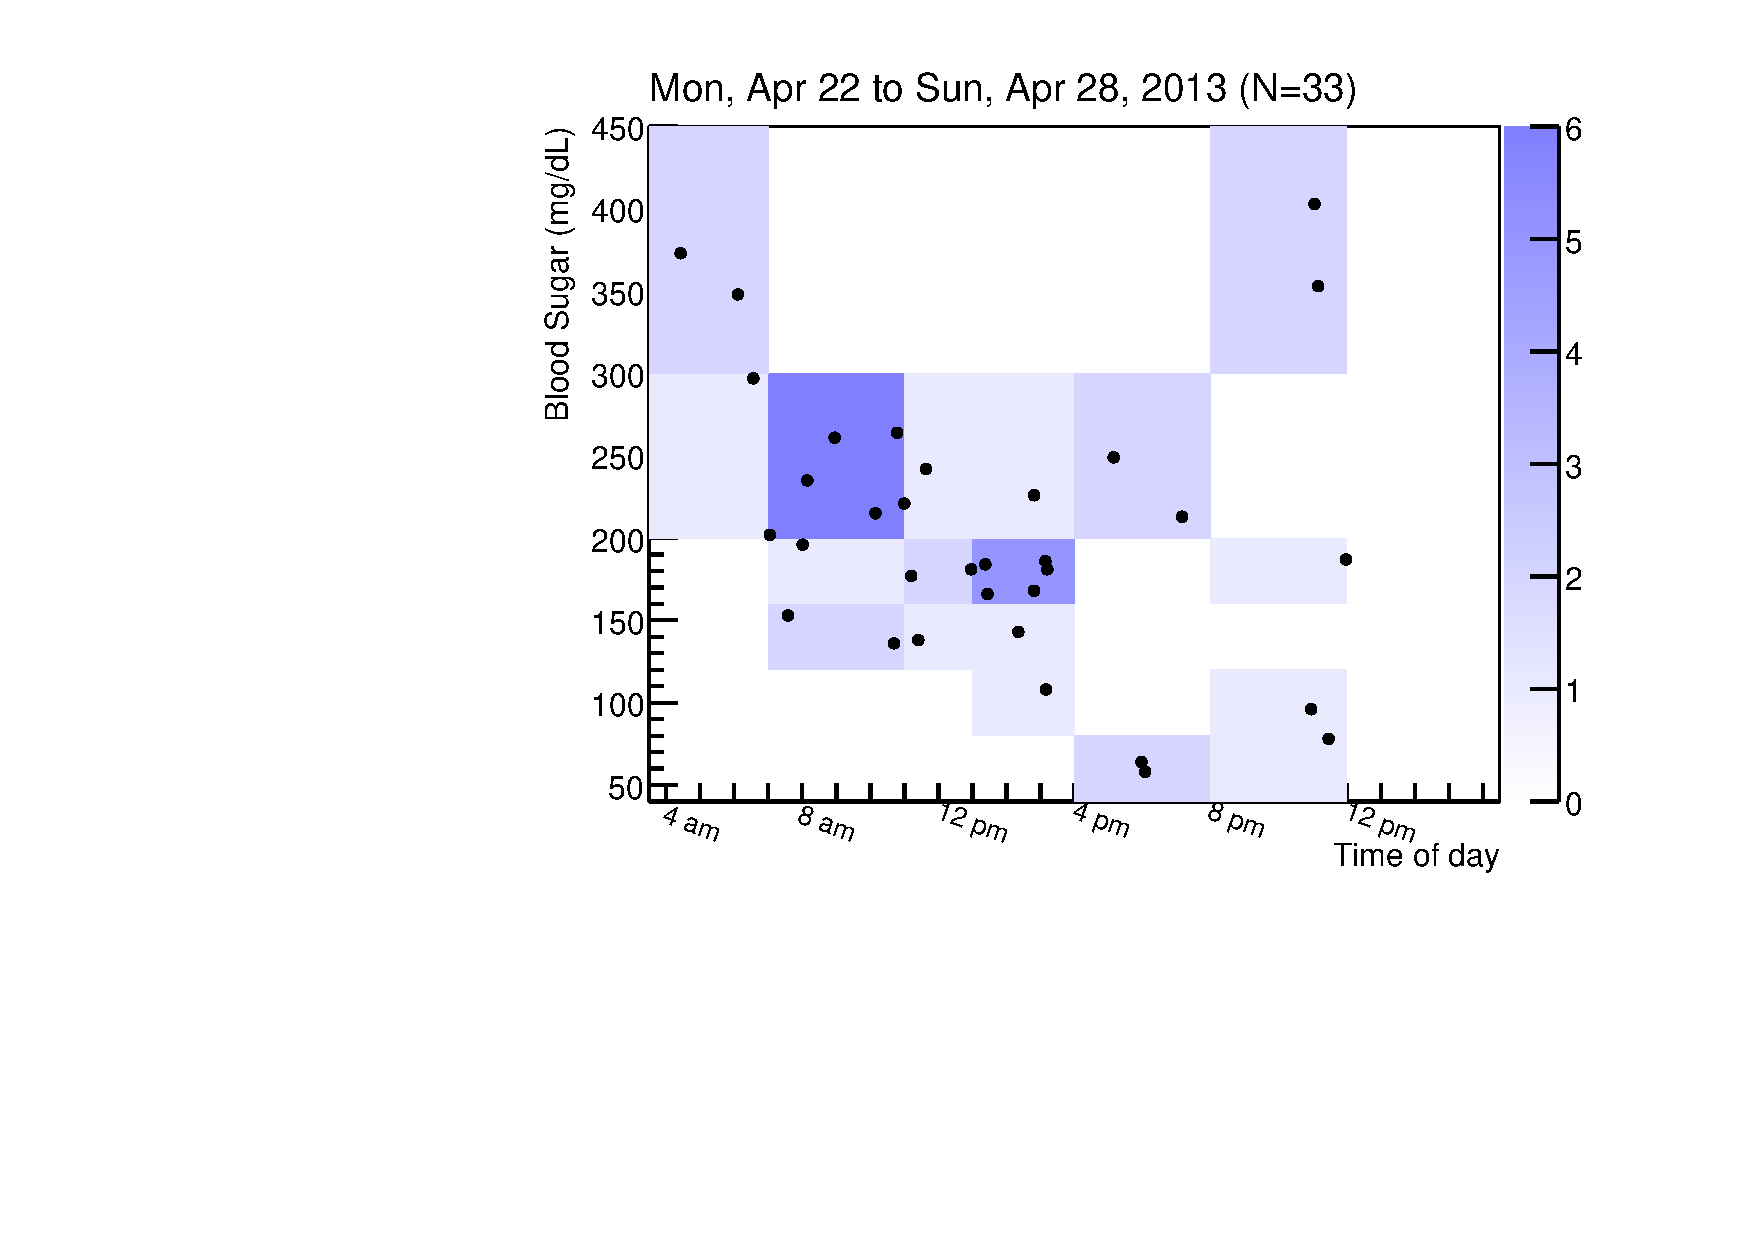
\includegraphics[width=4.5in]{figures/example_weekly.pdf}
\caption{An example scatter plot, with a coarse binning underneath, highlighting general trends in 
blood sugar levels for one week. These plots are intended to catch large trends in insulin dosage 
response.}
\label{default}
\end{center}
\end{figure}

\subsection{Conversions, conventions and formulas}

In the following, $U$ will refer to units of insulin; $S$ refers to sensitivity (in units of \sens).

\begin{table}[htdp]
\caption{Relevant Quantities}
\begin{center}
\begin{tabular}{|l|c|c|c|} \hline
Quantity & Abbrev. & Unit & Conversion to \mgdl \\ \hline
Measured blood sugar & $B_\text{meas}$ (or $B$) & \mgdl & - \\ \hline
Sensitivity & $S$ & $\mgdl\over{U}$ & - \\ \hline
Insulin-Carb Ratio & \carbratio & ${\text{g}\over U}$ & - \\ \hline
Food (carbs) & $C_0$ & grams & $B_f=C_0\cdot S/\ric$ \\ \hline
Active insulin time & $t_A$ & hours & - \\ \hline
Basal Rate & \rbas & $\mgdl\over h$ & $B_\text{bas} = \rbas\cdot t$ \\ \hline
\end{tabular}
\end{center}
\label{table:quants}
\end{table}%

In determining the insulin absorption function, several conditions must be met:
\begin{enumerate}
	\i At $t=0$, insulin is being rapidly absorbed.
	\i At infinite time, no more insulin will be absorbed.
	\i At $t=t_A$, all but 5\% of the insulin is absorbed.
\end{enumerate}

The last of these is chosen somewhat arbitrarily. The Minimed bolus wizard's ``active insulin time'' 
setting allows for seven options: 2-8 hours, in increments of 1 hour. It is not clear how Minimed 
defines active insulin time, but the third condition is seen as a reasonable approximation. In 
theory, one could determine this by reverse-engineering the ``active insulin remaining'' detail in the 
bolus wizard data.

Then, given these conditions, the quick-and-dirty simplest formula is:
\begin{equation}
\frac{{I}(t)}{I_0} = 1 - 0.05^{\left({t\over{t_A}}\right)^2} 
= 1-\exp\left( \ln(0.05)\cdot  \left({t\over{t_A}}\right)^2\right)
\end{equation}

Then
\begin{equation}
{B_I}(t) = -S\cdot I_0\left( 1 - 0.05^{\left({t\over{t_A}}\right)^2} \right)
\label{eq:insulin}
\end{equation}

Taking derivatives of this yields:
\begin{equation}
\pderiv{B_I}{t} = -6SI_0\frac t{t_A^2} 0.05^{\left(\frac t{t_A}\right)^2}
\comma
\pderiv{^2 B_I}{t^2} = SI_0\cdot0.05^{\left(\frac t{t_A}\right)^2}\left({36t^2\over t_A^4} - {6\over t_A^2} \right)
\end{equation}
Setting the 2nd derivative to 0, we can get the maximum $dB/dt$, $t\sim \frac {t_A}{\sqrt{6}}=1.63$ 
hours for $t_A=4$ (at which point $dB/dt=0.37I_0$ u/hr), 0.81 hours for $t_A=2$. 

Fig.~\ref{fig:absorption} shows the total absorption and $dB/dt$ of a typical ``4-hour'' insulin bolus.

\begin{figure}[htbp]
\begin{center}
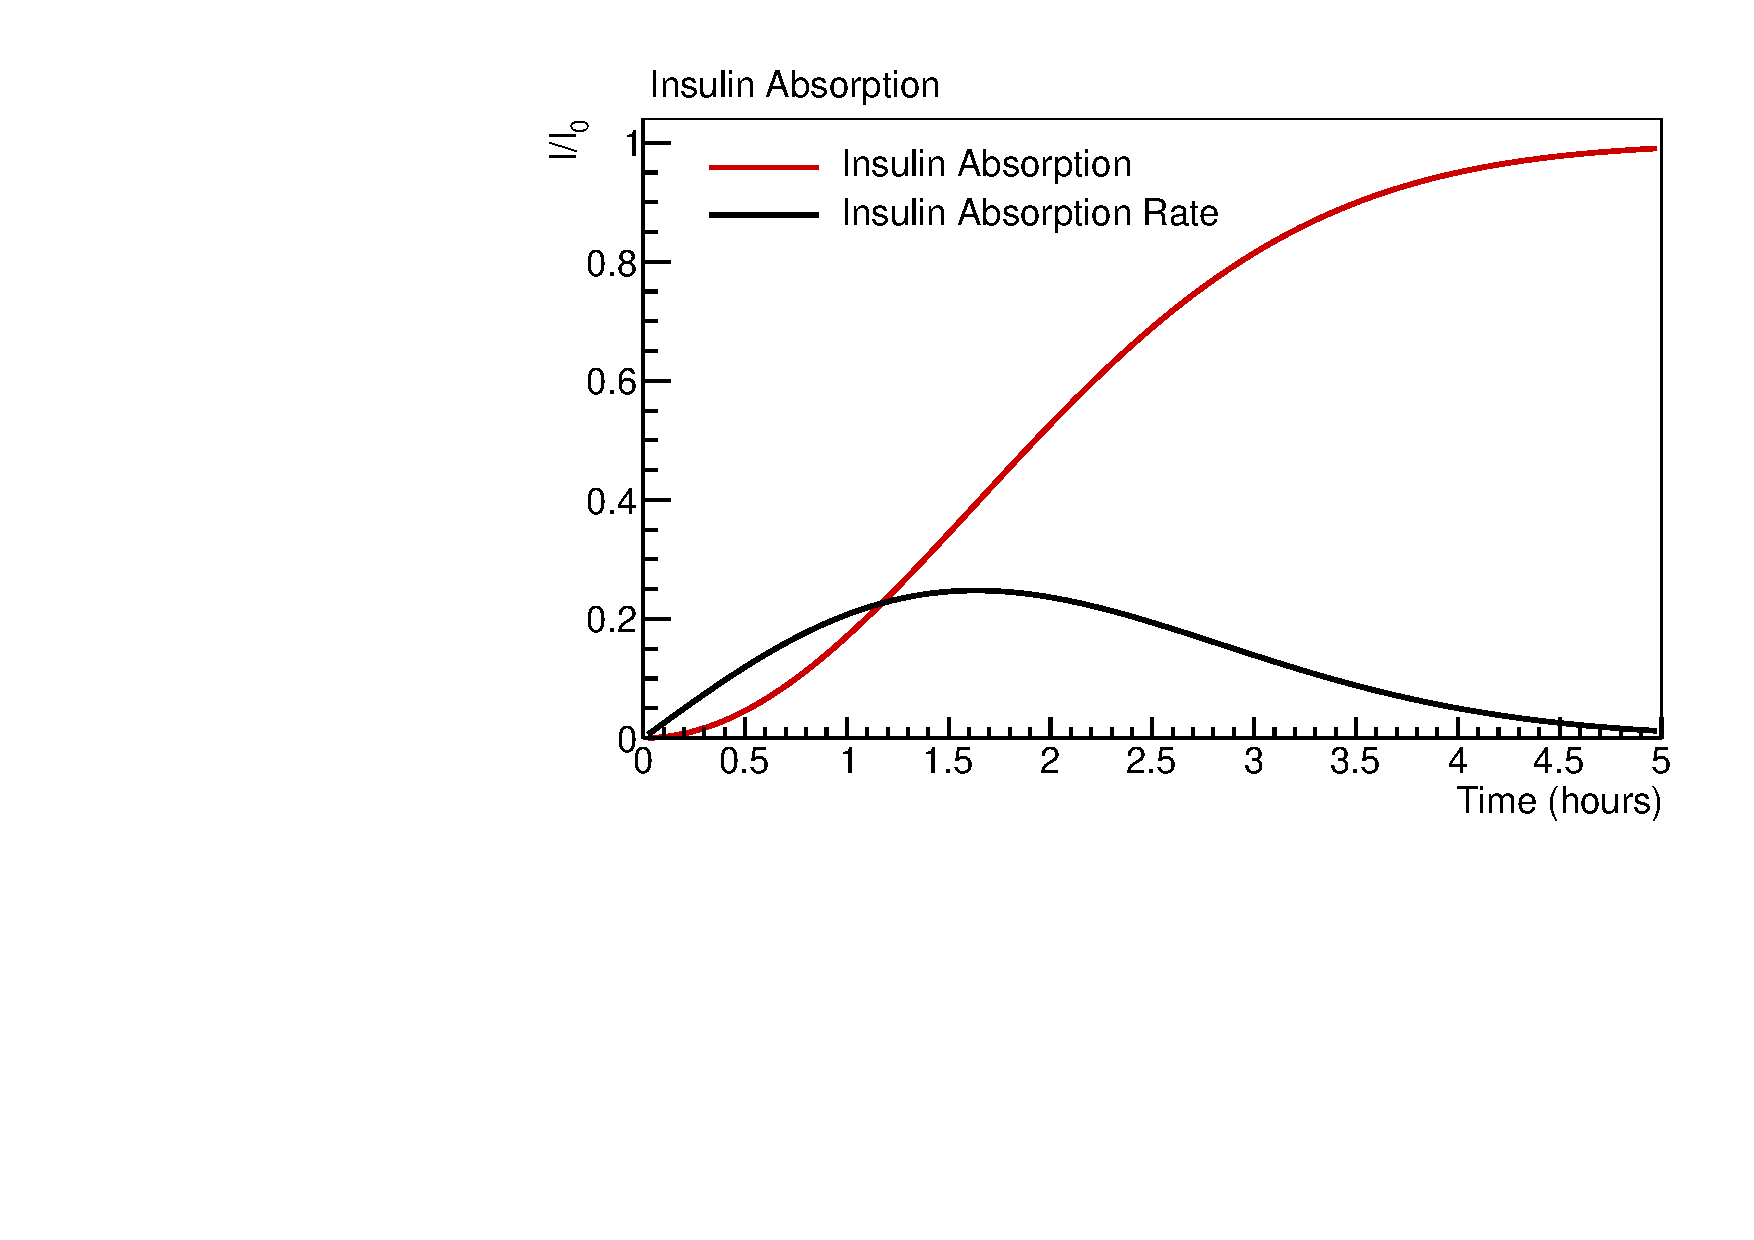
\includegraphics[width=4.5in]{figures/absorption.pdf}
\caption{Insulin absorption curves. The red curve is the overall fractional absorption over time 
($I/I_0$), and the black curve is $dI/dt$. The curve is plotted with $t_A=4.0$, meaning that 95\% of 
the insulin is absorbed after 4 hours.}
\label{fig:absorption}
\end{center}
\end{figure}

Food absorption rates follow the same reasoning. Here, however, the $t_A$  equivalent (call it $t_C$) 
varies according to the food's score on the glycemic index. Thus, we set $t_C=2.0$ hours for 
simplicity. Thus:

\begin{equation}
{B_C}(t) = {S\over\ric}\cdot C_0\left( 1 - 0.05^{\left({t\over{t_C}}\right)^2} \right)
\label{eq:carb}
\end{equation}

\subsection{How the predictive plot macro works.} 

Rather than looking at raw BG readings, carb totals, and correction boluses, it would be easier to 
look at all of these quantities in their shared units: BG concentration. As described in the table 
\ref{table:quants}, there are conversion factors to translate each quantity into a BG-equivalent. 
Of course, some of these conversions include ``unknown'' quantities - the very quantities we are 
trying to determine. Thus, the plot will represent a user's estimate, based on his settings.

\begin{figure}[htbp]
\begin{center}
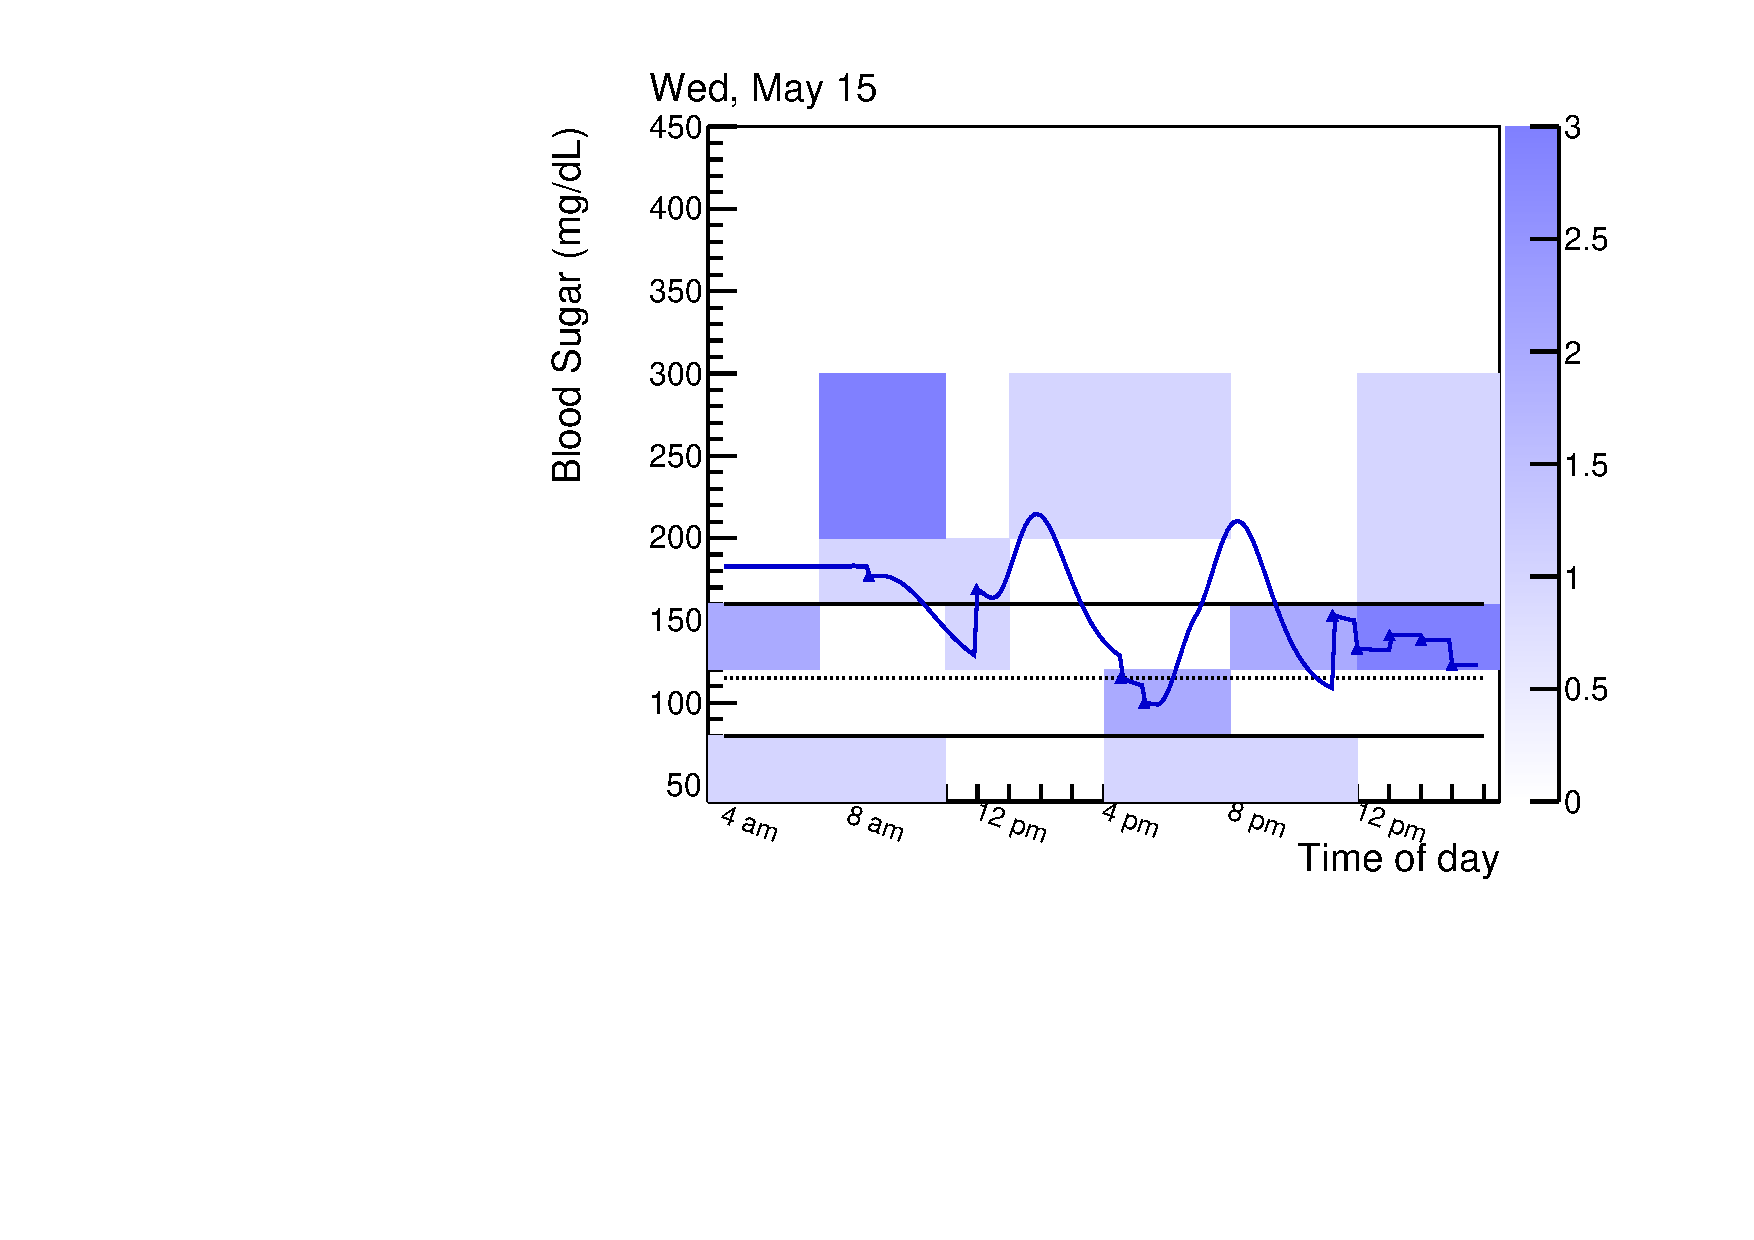
\includegraphics[width=4.5in]{figures/example_predictive.pdf}
\caption{Predictive curve overlaid on top of BG measurements. The curve resets each time a new 
measurement is made. From the plot above, one can see problems with the morning regime, as well as 
the evening regime. 
}
\label{fig:predictive}
\end{center}
\end{figure}

The plot macro (see fig. \ref{fig:predictive}) uses 3 classes of information: BG measurements, food 
intake, and insulin dosages. Based on $S$, $\ric$ and $t_A$ at the time of the event, it uses 
eq. \ref{eq:insulin} and \ref{eq:carb} (or rather their derivatives) to estimate the BG evolution 
over time, given the user's inputs. When an additional BG measurement is made (it is taken to have 0 
uncertainty), any discrepancy between the estimate and the new measurement is an indication of an 
incorrect dosage (whether caused by sensitivity $S$, food estimate $C_0$, basal rates, or 
insulin-to-carb ratio ($\ric$), or a combination of these. The discontinuity in the graph represents 
the magnitude of the discrepancy.

The usefulness of an isolated plot like this is limited. One cannot, given one measurement in time, 
determine which dose-related quantity ($S$, $C_0$, $\ric$, \rbas) is incorrect. One can circumvent 
this problem in 2 ways: 1. Reduce the number of unknowns by refraining from eating, or not issuing 
a corrective bolus, and 2. Analyze data over multiple days, with different characteristics (more 
food / less food, etc). 

It is also important to remember that a predictive curve which lines up exactly with the measured 
BG could be caused by the cancellation of 2 or more effects.

\subsection{Predictive plot macro and error bands.} More on this later.

\section{Long-term trends}

\begin{figure}[htbp]
\begin{center}
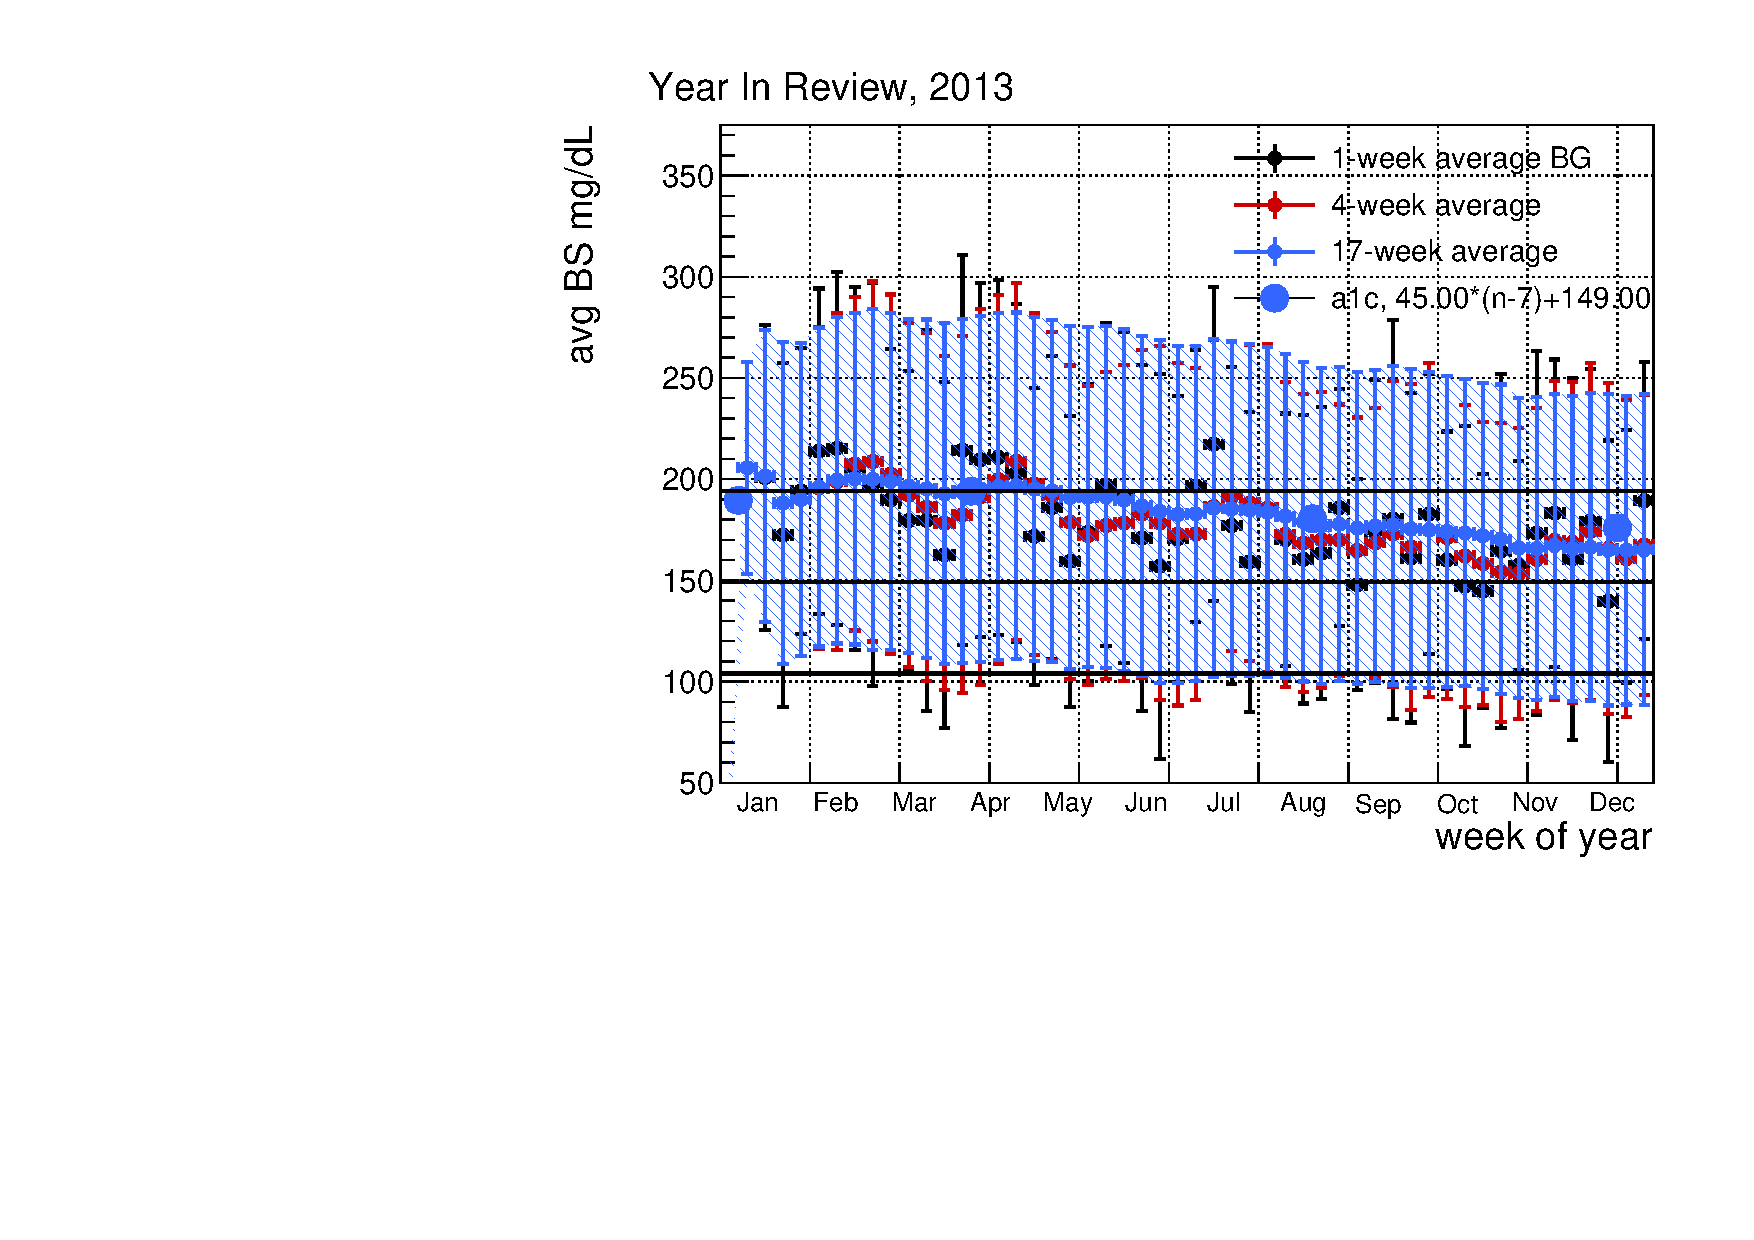
\includegraphics[width=4.5in]{figures/year_in_review_2013.pdf}
\caption{Year in review for the year 2013. Detailed record-keeping began in May.
\hbac values shown are 7.9, 8.0, 7.7, and 7.6.
}
\label{fig:year}
\end{center}
\end{figure}

An important aspect of management is assessing long-term trends. Fig.~\ref{fig:year} is a year-long 
review, which includes rolling 1-week averages, 4-week averages, and 17-week averages. (17 weeks is 
roughly the lifetime of a red blood cell, and thus the 17-week average should give a fair comparison 
to \hbac.) 

\section{Phase I Software}

\subsection{Dedicated Event-by-event macros}

User-conducted studies are foreseen to play a large role in the Phase I software. The fasting basal 
rates and fixed carbohydrate meals are extremely valuable, and as such, making them easy for the user 
to execute is an important goal of the software.

For somewhat unrelated reasons, a skeleton of a user interface has been developed to help keep track 
of certain data. This user interface could allow the user to indicate when such a study (fixed carb 
or fasting basal) has been performed, rather than the software attempting to find these events on 
its own.

It is envisioned that in the Phase III version of the software will have the capacity to find these 
events, and other ``accidental studies'' unwittingly carried out by the user, and act on them. 
However, the aforementioned user-delimited studies will suffice; they are also safer, since the Phase 
III software would require the user to keep more detailed records.

%% \section{Phase I.5}

%% In this phase, specific events are plotted in order to get a feel for the meaning of data branches 
%% (not always ), and to gain experience ahead of developing the phase II software.

%% \begin{enumerate}
%% \item What does BWZActiveInsulin mean with a value of -1?
%% \end{enumerate}

\section{Phase II Software}

\subsection{Food uncertainties}

A crucial aspect of the Phase II software would be to incorporate carbohydrate  uncertainties into the 
data model. Consider this scenario: each time a packaged, labeled food is consumed, the dosage is 
correct; however, each time an un-labeled meal is consumed, the insulin dosage is underestimated, 
leading to higher blood sugar levels. The Phase I software will suggest increasing bolus rates, and 
as a result the average blood sugar will decrease. However, well-labeled meals will now be 
consistently overestimated.

\subsection{The Event Data Model (EDM)}

It is not altogether straightforward how to specify an ``event'' in this type of scenario. Several 
things could qualify as ``events,'' in that they happen at a particular time: a glucose measurement, 
a meal, and a bolus. Sometimes these events occur simultaneously, and sometimes they do not. Some 
events, such as exercise and raised basal rates, occur over a fixed period of time. And the act of 
insulin absorption and carbohydrate metabolism evolve over a period of time.

Since the goal of the software is to suggest changes in insulin dosages, it makes sense to build the 
event around the suggested change in dosage (``At this time, change your bolus rate from 15 g/unit 
to 18 g/unit''). 

\section{Phase III Software}

\section{Pairing with dietary changes}
It has been suggested that coupling an appropriate insulin regimen with dietary changes may 
significantly improve sugar control. ADA suggestions, along with a pre-prandial test of $<$130, 
a post-prandial target of $<$180 is desired. It is likely that this can only be achieved with 
significant dietary changes. These changes include (but are not limited to):
\bi
	\i Reducing total carb intake (weekly metric)
	\i Spreading carb intake over a longer period of time (coupled with an early bolus!)
	\i Surrounding oneself with low-carbohydrate food.
\ei

List of foods no longer desirable as a full meal:
\bi
	\i Spaghetti
	\i Rice
	\i Bread
	\i Cookies
	\i Ooh, cereal. Well well well.
	\i Basically anything above 50 (?) grams of carb - {\it unless} it is low on the glycemic index
\ei

Replacement options
\bi
	\i Dark chocolate
	\i Vegetables
\ei

A reasonable target might be to never be above 200 mg/dL. Particularly in the post-prandial period, 
from which I have managed to shift all testing. Other healthy habits:
\bi
	\i Drink lots of water
	\i Exercise
	\i Avoid stress
	\i Vitamins?
\ei

\subsection{Quantifying the Advantages of Carb Intake Reduction and E.B.}

Fig.~\ref{fig:reduceCarb_eb} has some representative plots showing the potential gain of reducing 
carb intake, and bolusing before food intake (early bolus). The plots show the gains assuming perfect 
bolus estimates, however it should be noted that lowering carbohydrate intake can also reduce the 
potential for mis-estimation. Strict adhesion to a $<$65 grams per meal diet with heavy early-bolus 
could result in as much as a 1\% improvement in \hbac

\begin{figure}[htbp]
\begin{center}
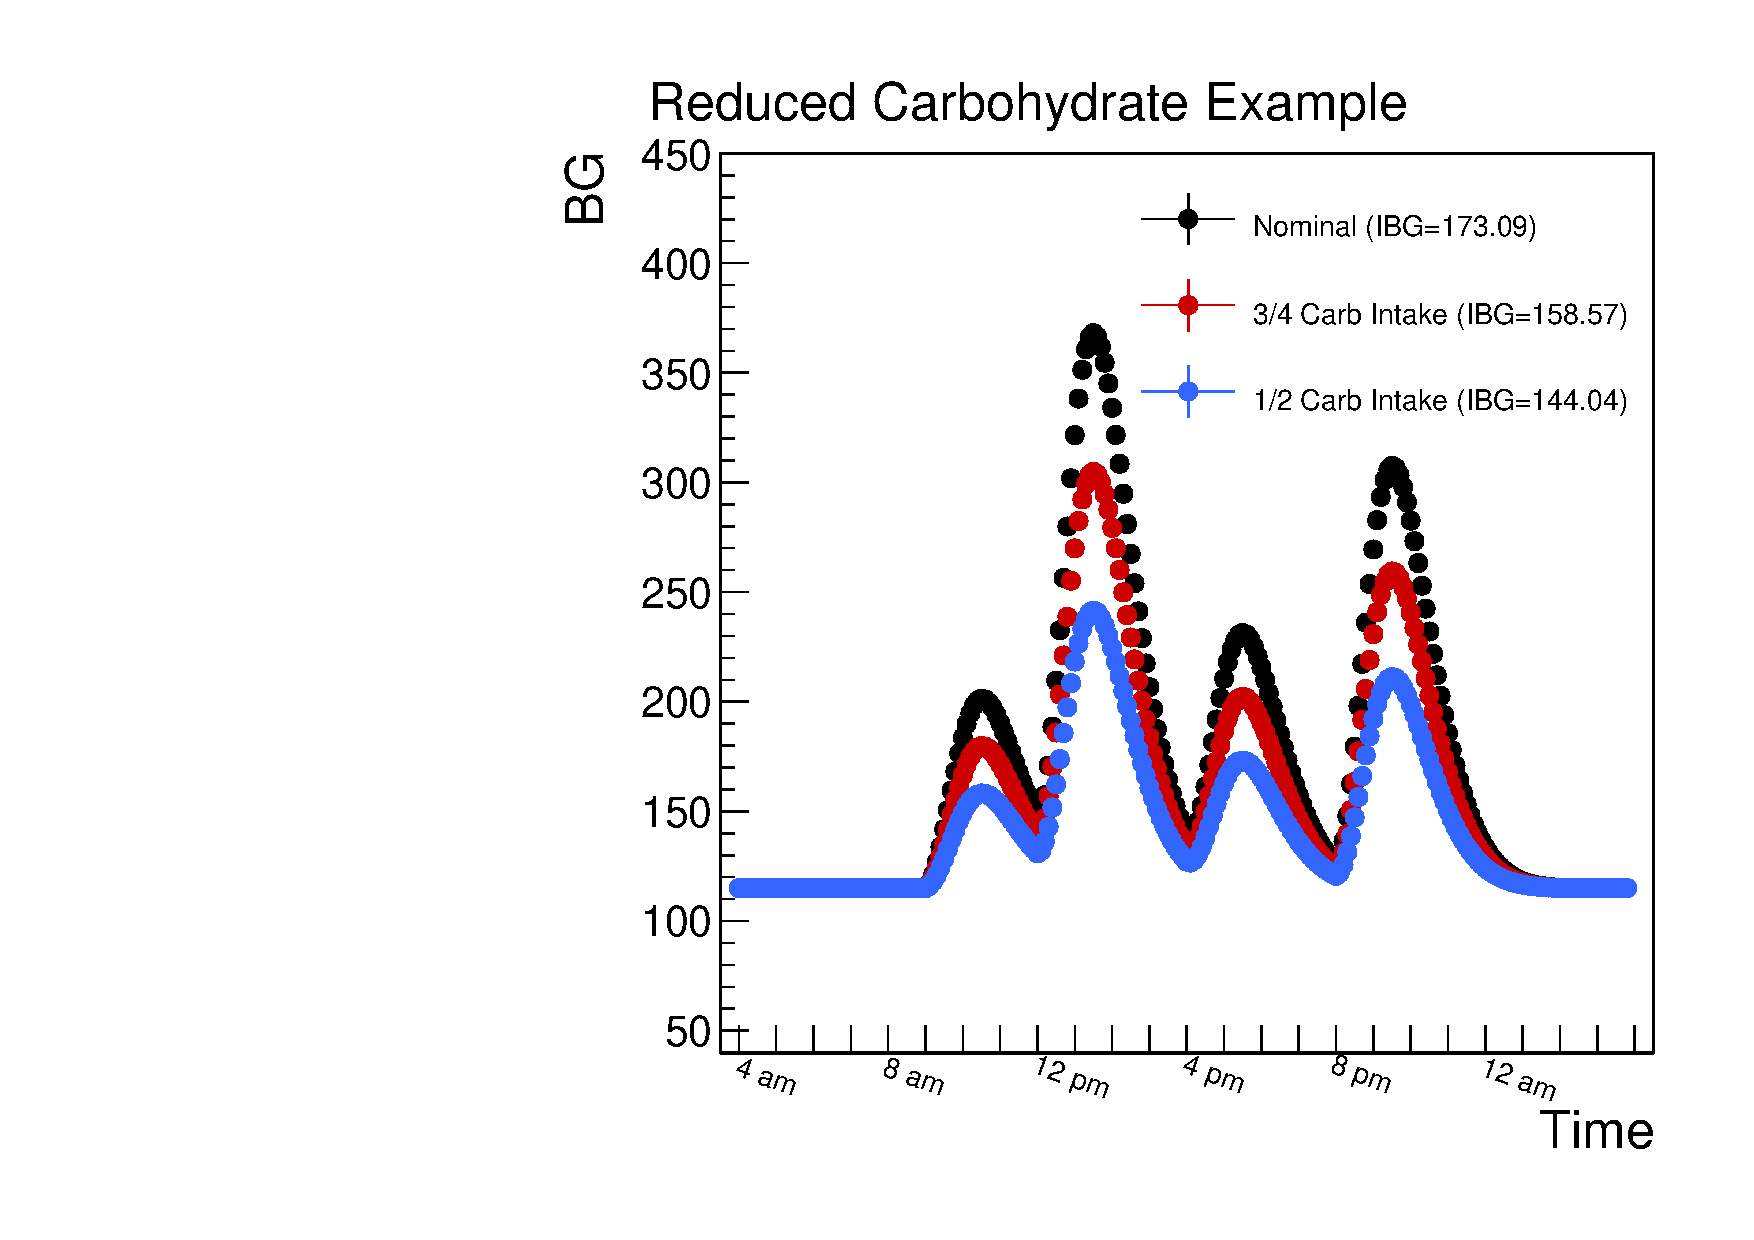
\includegraphics[width=3.in]{figures/reduced_carb.pdf}
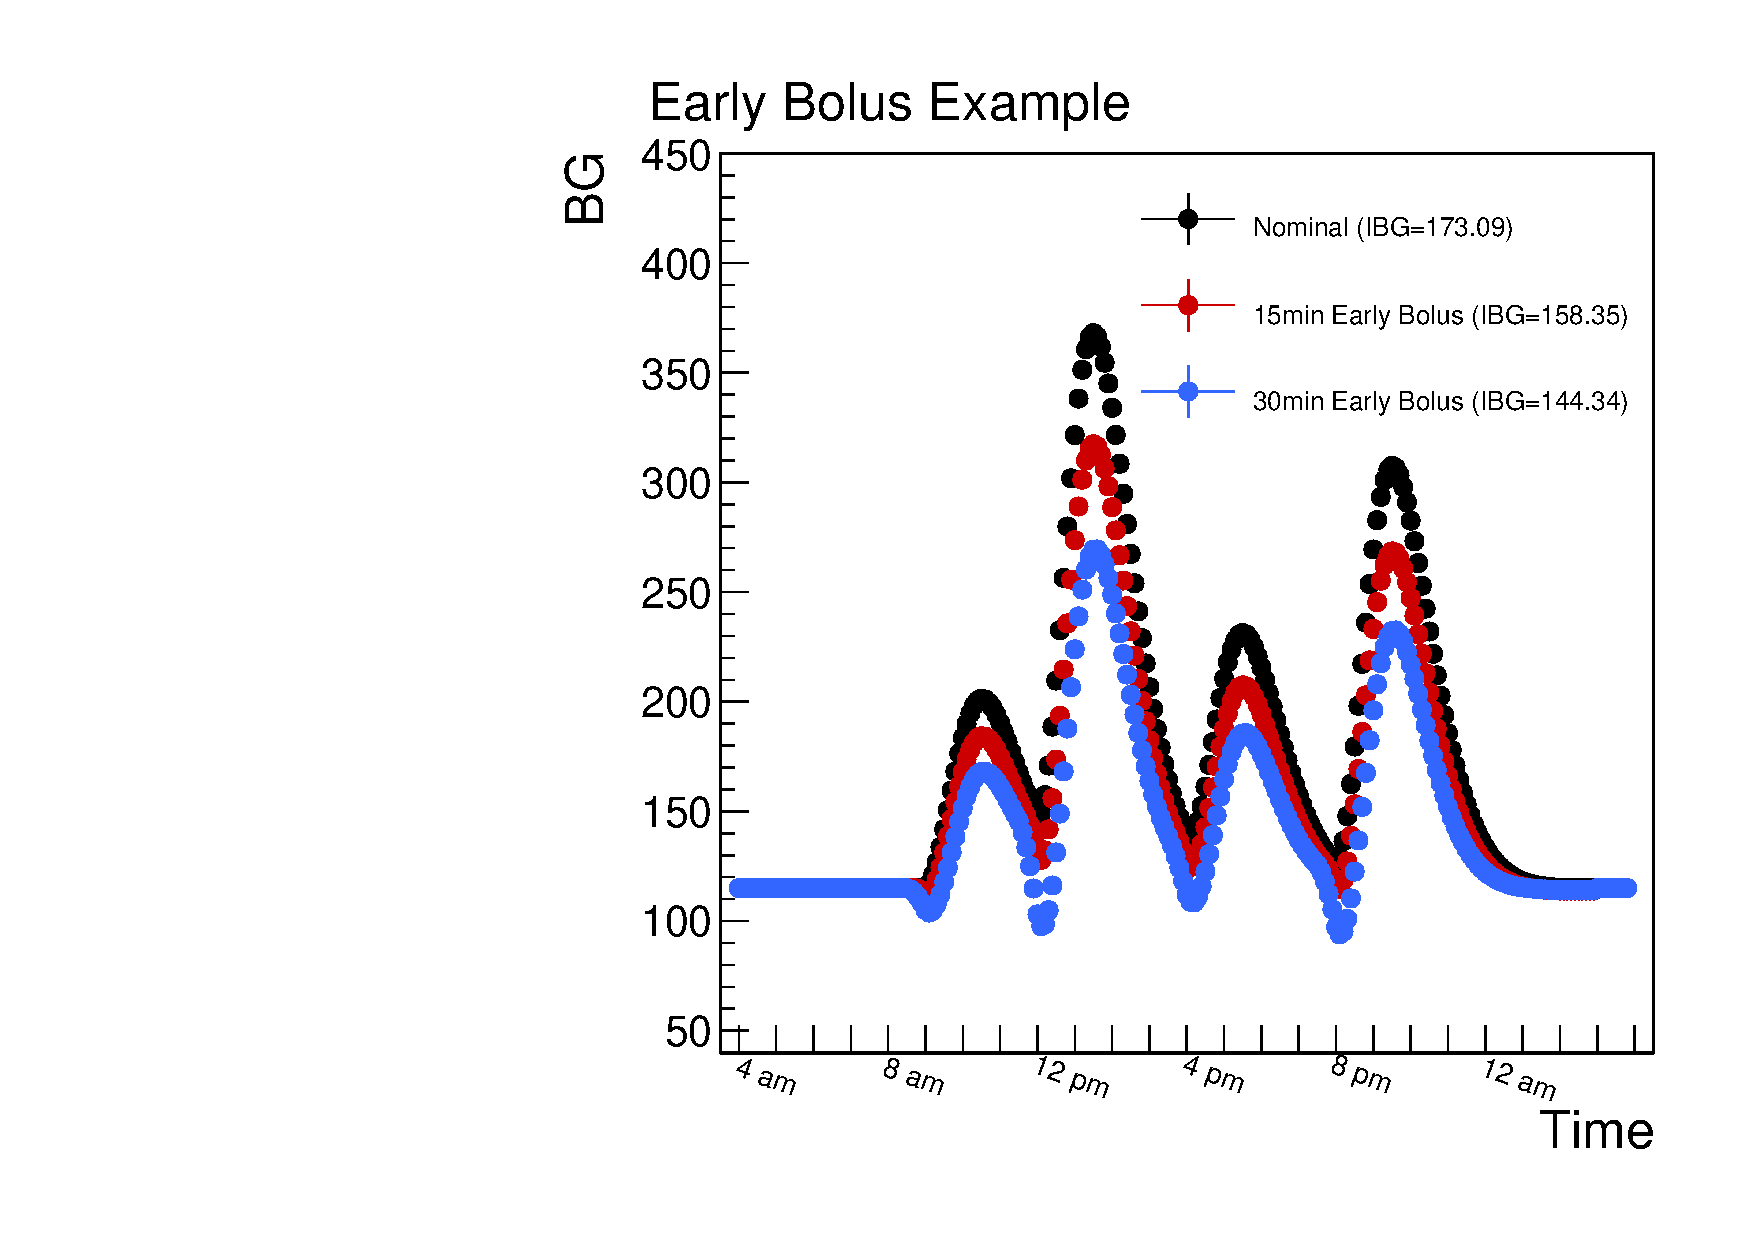
\includegraphics[width=3.in]{figures/early_bolus.pdf}
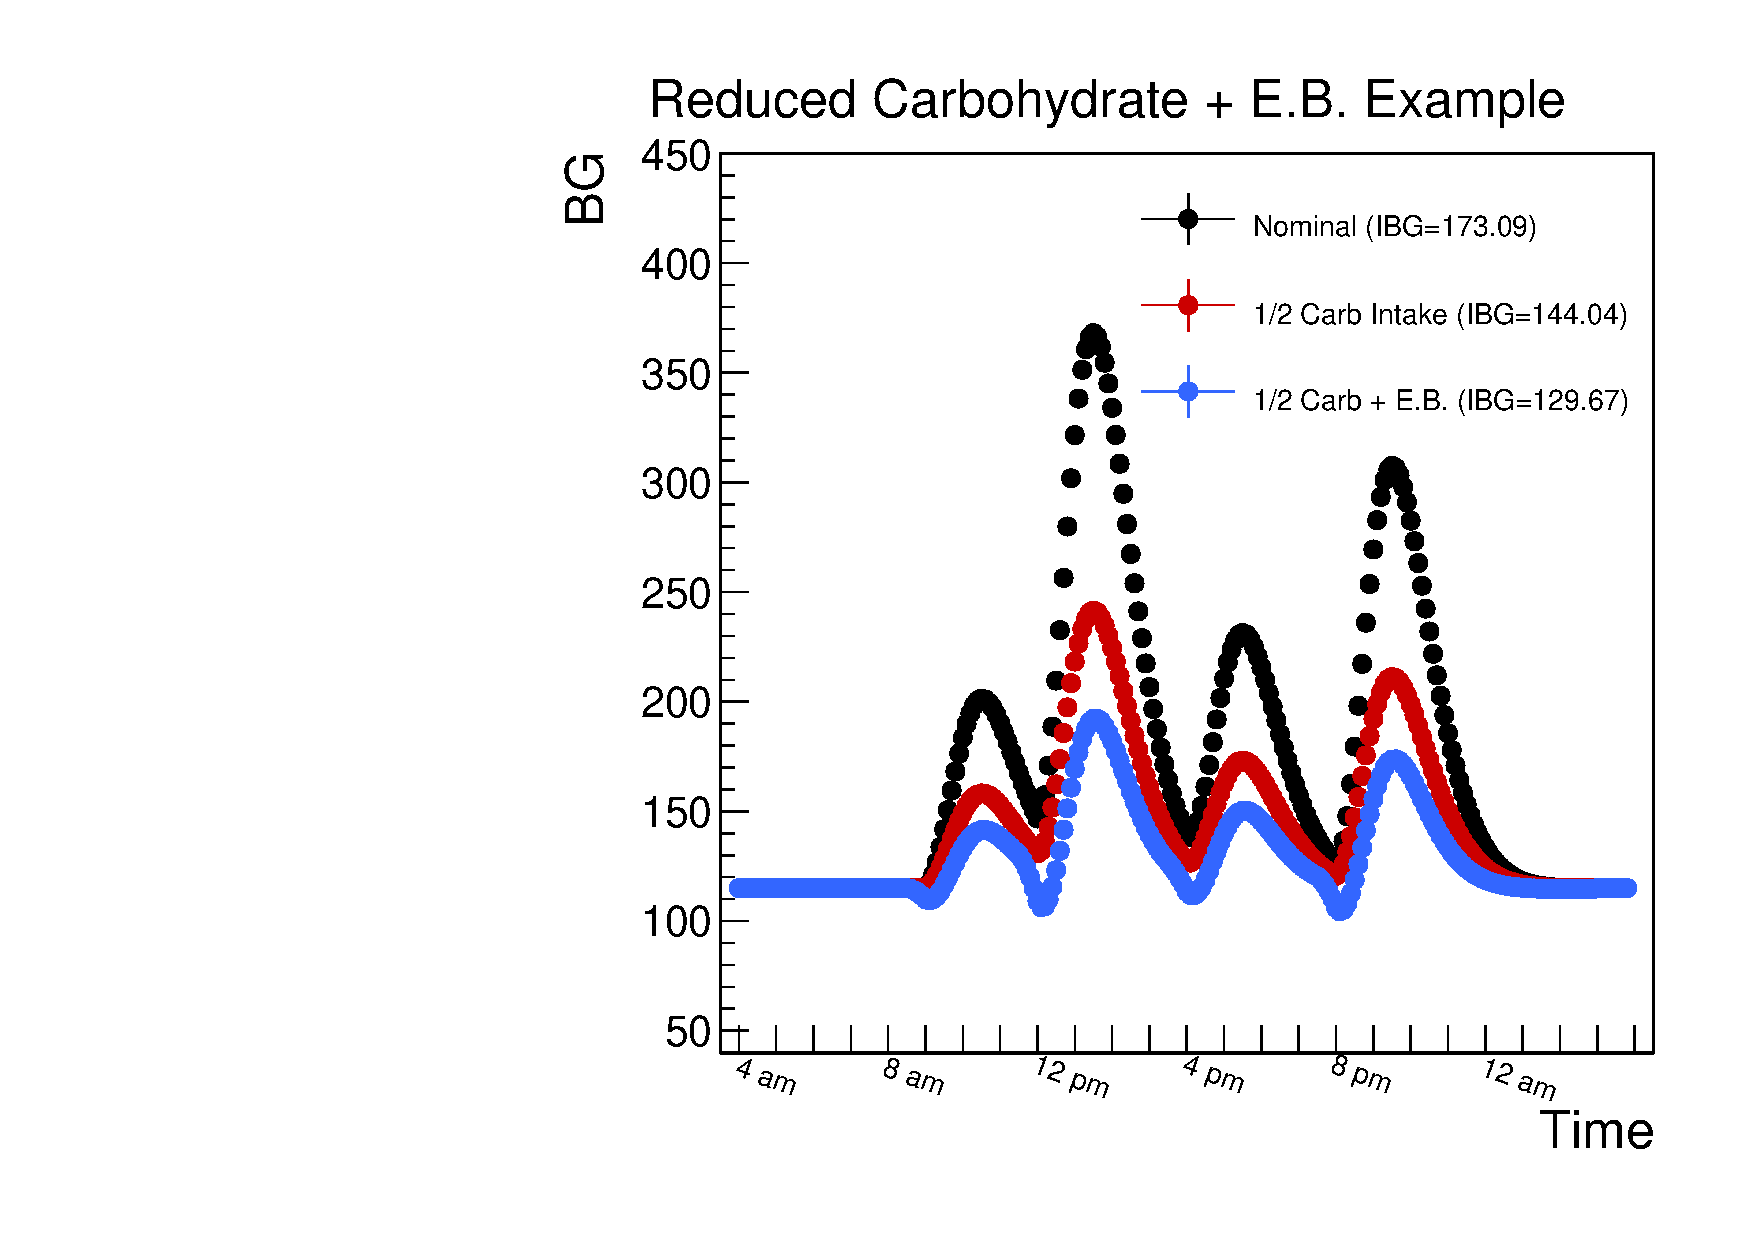
\includegraphics[width=3.in]{figures/reduced_carb_eb.pdf}
\caption{Left: The effects of multiplying carbohydrate intake by a factor of 3/4 and 1/2 on a 
nominal day's BG readings. 
Right: The effects of early bolus, by 15 minutes and 30 minutes. Bottom: Combining both methods. 
Plots are based on a 2-hour glucose absorption rate and a 4-hour insulin absorption rate.
The nominal day consists of 45g at 9am, 130g at 12pm, 60g at 4pm and 100g at 8pm. }
\label{fig:reduceCarb_eb}
\end{center}
\end{figure}


\section{Additional Studies}

\subsection{Fasting basal rates (Recurring)}

This recurring study is an integral part of the Phase I 

\subsection{Fixed-carbohydrate meals (Recurring)}

This study is also important to phase I. The goal is to consume a meal with a fixed, 0-uncertainty 
number of carbohydrates.

\subsection{Clean Correction Bolus studies}

Correcting a large BG deviation (300+) can give an excellent handle on insulin sensitivity, a key 
number that affects the correction estimates of both $\rbas$ and $\ric$. (Must assume a reasonably 
accurate basal rate.) The sensitivity is essential for setting error bars on BG extrapolation curves.

\subsection{Effect of coffee on blood sugar levels}

It is hypothesized that coffee intake should be accompanied by an insulin bolus, though there is 
insufficient data to corroborate this. A study is suggested which probes the effect of coffee, on an 
empty stomach, during a period with well-known stable basal rates.

\subsection{Effects of fatty foods}

\subsection{Effect of alcohol}

\section{Personal Insulin Dose Changes}

\subsection{Notes}

Important note: the process of correcting insulin doses is highly sensitive to the sensitivity number, 
$S$. Note that it figures in to carb ratios, insulin, basal rates and correction boluses. Thus, if 
$S$ is underestimated while trying to change basal rates, the magnitude of the change in basal rate 
will be overestimated.

One way to probe $S$ is to have a clean, non-food correction bolus after a high (say 300+) glucose 
reading. The subsequent measurement is influenced almost entirely by the correction bolus, and can 
be used as a data point for that 3-hour period.

The ``1500 rule'' (as described in the literature, applying to fast-acting insulin) is supposed to 
relate daily insulin totals to sensitivity, i.e. $S=1500/T$. I am not sure whether this is based off 
a 2000 calorie diet, and whether or not eating more changes this value. In any case, my daily totals 
range from 30-50, so sensitivity, accordingly, seems to be anywhere from 30 to 50. Or 65, who knows?

\subsubsection{Relation between average glucose readings and \hbac}
There is some description in the literature about relating \hbac to average BS.
\footnote{See http://care.diabetesjournals.org/content/25/2/275.full}
Based on this one text, the formula is below:
\[
BS(\mgdl)=(35.6 \times \hbac)-77.3
\]
or, reframing in a way which emphasizes the 
\[
BS(\mgdl)=35.6\times(\hbac-7)+171.90
\]
The ADA has a much more pessimistic estimate (link?):
\[
BS(\mgdl)=28.71\times(\hbac-7)+154.42
\]
This number may depend on the nature of blood sugar measurement (relating to how long after eating
each measurement is taken) - and thus might depend on one's personal habits. Trying to correlate
my personal BS (taken from a 17-week rolling average) with my \hbac readings, the relationship is
roughly
\[
BS(\mgdl)=45.0\times(\hbac-7)+149.0
\]

Below are some representative numbers, for the purposes of setting targets. Roughly speaking, it 
appears as if 1/4 of a point in \hbac is equivalent to 9 \mgdl~(paper), 7 \mgdl~(ADA), 11 
\mgdl~(personal). \\
\begin{center}
\begin{tabular}{|c|c|c|c|}
\hline
\hbac & BS (Paper) & BS (ADA) & BS (Personal) \\ \hline
6.50  & 154.1      & 140.1    & 126.5         \\ \hline
6.75  & 163.0      & 147.2    & 137.8         \\ \hline
7.00  & {\bf 171.9}      & {\bf 154.4}    & \bf{149.0}\\ \hline
7.25  & 180.8      & 161.6    & 160.2         \\ \hline
7.50  & 189.0      & 168.8    & 171.5         \\ \hline
7.75  & 198.0      & 176.0    & 182.8         \\ \hline
8.00  & 207.5      & 183.1    & 194.0         \\ \hline
8.25  & 216.4      & 190.3    & 205.2         \\ \hline
8.50  & 225.3      & 197.5    & 216.5         \\ \hline
\end{tabular}
\end{center}

\subsection{Evolution of Carb Ratios}

\begin{table}[h]
\caption{Carb Ratios}
\footnotesize
\begin{center}
\begin{tabular}{|c|c|c|c|c|c|c|c|c|c|c|c|c|c|c|c|c|c|c|c|c|c|c|c|c|}
\hline
Date       & 12am & & & & 4am & & &    & 8am & & & & 12pm & & &    & 4pm &    & & & 8pm & &    & 11pm \\ \hline
2013/01/01 & 18   & & & &     & & &    & 16* & & & & 15   & & &    &     & 16 & & &     & &    &      \\
2013/06/12 & 18   & & & &     & & & 16 &     & & & & 14*  & & &    &     & 16 & & &     & &    &      \\
2013/06/20 & 16   & & & &     & & & 16 &     & & & & 14*  & & &    &     & 16 & & &     & & 15 &      \\
2013/10/18 & 16   & & & &     & & & 16 &     & & & & 14*  & & & 16 &     & 16 & & &     & & 15 &      \\
2014/05/22 & 16   & & & &     & & & 16 &     & & & & 19*  & & & 19 &     & 19 & & &     & & 19 &      \\
2014/05/23 & 16   & & & &     & & & 16 &     & & & & 16*  & & & 16 &     & 16 & & &     & & 16 &      \\
2014/05/27 & 16   & & & &     & & & 16 &     & & & & 17*  & & & 19 &     & 20 & & &     & & 18 &      \\
%          %      & & & &     & & &    &     & & & &      & & &    &     &    & & &     & &    &      \\
\hline
\end{tabular}
\end{center}
\label{default}
\end{table}%
Where * means ``actually starts 1/2 hour earlier.''

\begin{table}[h]
\caption{Sensitivity}
\footnotesize
\begin{center}
\begin{tabular}{|c|c|c|c|c|c|c|c|c|c|c|c|c|c|c|c|c|c|c|c|c|c|c|c|c|}
\hline
Date       & 12am & & & 3am &    & &6am & &    & 9am & & & 12pm & & & 3pm &    & & 6pm & &    & 9pm &    & 11pm \\ \hline
2013/01/01 & 60   & & &     & 60 & &    & & 40 &     & & & 35   & & &     & 35 & &     & & 40 &     & 60 &      \\
2013/06/12 & 60   & & &     & 60 & &    & & 40 &     & & & 35   & & &     & 50 & &     & & 40 &     & 60 &      \\
2013/06/12 & 60   & & & 60  &    & & 45 & &    & 45  & & & 45   & & & 50  &    & & 45  & &    & 60  &    &      \\
2013/06/13 & 60   & & & 60  &    & & 65 & &    & 65  & & & 50   & & & 50  &    & & 45  & &    & 60  &    &      \\
2013/10/18 & 60   & & & 60  &    & & 65 & &    & 65  & & & 50*  & & & 50  &    & & 45  & &    & 60  &    &      \\
2014/05/22 & 60   & & & 60  &    & & 65 & &    & 65  & & & 65*  & & & 65  &    & & 65  & &    & 60  &    &      \\
%    & & & &     & & &    &     & & & &      & & & &     &    & & &     & & &      \\
\hline
\end{tabular}
\end{center}
\label{default}
\end{table}%

\begin{table}[h]
\caption{Basal Rates}
\footnotesize
\begin{center}
\begin{tabular}{|c|c|c|c|c|c|c|c|c|c|c|c|c|c|c|c|c|c|c|c|c|c|c|c|c|}
\hline
Date       & 12am & &    & & 4am & &    & & 8am & &    & & 12pm & &     &     & 4pm & &    & & 8pm & &    & 11pm \\ \hline
2013/06/12 & .8   & & .8 & & .9  & & .9 & & .9  & & .9 & & .9   & & .85 &     & .85 & & .9 & & .9  & & .9 &      \\
2014/03/30 & .8   & & .8 & & .9  & & .9 & & .9  & & .9 & & .9   & & .85 & .75 &     & & .8 & & .9  & & .9 &      \\
2014/05/22 & .8   & & .7 & & .7  & & .7 & & .9  & & .9 & & .9   & & .85 & .75 &     & & .8 & & .9  & & .9 &      \\
2014/05/26 & .8   & & .75& & .75 & & .75& & .9  & & .9 & & .9   & & .85 & .75 &     & & .8 & & .9  & & .9 &      \\
%    & & & &     & & &    &     & & & &      & & & &     &    & & &     & & &      \\
\hline
\end{tabular}
\end{center}
\label{default}
\end{table}%

\subsection{Log of changes}
Started Wednesday, June 12, 2013.

\begin{table}[htdp] % htdp
\begin{center}
\begin{tabular}{|p{1in}|p{5in}|}
\hline
2013/6/12  & Increased basal 0.1 u/hr, 8am-12pm (from 0.8 to 0.9). Actual estimate was 1 u/hr. Need to increase in steps if not effective. {\bf Hindsight: estimate was too high due to low sensitivity!} \\
           & Decreased lunchtime $C$ from 15 to 14 g/u carb ratio. May not be enough. (May also be estimating food poorly.) Careful - sensitivity! \\
           & Changed sensitivity from 35 to 50 from 2pm-8pm, based on lows in the afternoon. This was the exact estimate. 
\\ \hline
2013/6/13  & Increased sensitivity to 65 in the morning, due to constant, high-significance lows. \\ \hline
2013/6/20  & Decreased carb:insulin ratio due to high reading with some cereal. \\ \hline
2013/10/18 & Increased carb:insulin ratio in the afternoon (3pm) due to persistent low readings. \\
           & Sensitivity change at 11:30am instead of 12pm to make it relevant for lunchtime boluses. \\ \hline
2014/03/30 & Decreased basal 0.1 u/hr between 3pm and 8pm, due to frequent lows (and a particular event in week 64 - 50 points in 2 hours). Other possible explanation: longer insulin act time? \\ \hline
2014/05/22 & Increased carb/insulin ratio in the afternoon and evening due to persistent lows. May have been too extreme - will see. \\ 
2014/05/22 & Decreased basal at night, after a precision measurement and some other lows. \\ \hline
2014/05/26 & Increased basal slightly as a tweak to the previous change \\ \hline
2014/05/27 & Increased carb:insulin ratio in the afternoon, after a very clean food event. (Estimate is 23 - changed to 20 at 5pm, with smoothness in between) \\ \hline
\end{tabular}
\end{center}
\end{table}%

\subsection{Specific food successes}
\begin{center}
\begin{tabular}{|p{2in}|p{4.5in}|}
\hline
2013/6/25 - Frozen Pizza & 120 g, plus 4 hours at 130\%. 127 \mgdl\ in morning. \\ \hline
\end{tabular}
\end{center}

\end{document}
